\documentclass[
	12pt,
	colorbacktitle,
	accentcolor=tud1c,
	draft,
	twoside,
	german
]{tudexercise}
% For Draft, make Report... for whatever reason normal draft doesnt work...
% ]{tudreport}

% USEPACKAGE
% changed counter for section wise counting
\usepackage{chngcntr}
\usepackage[utf8]{inputenc}
\usepackage[T1]{fontenc}
\usepackage[ngerman]{babel}
\usepackage{graphicx}
\usepackage{subcaption}
\usepackage{listings}
\usepackage{todonotes}


%% unused packages, might be useful someday
% linebreak for urls in bitexx
%\usepackage{url}
%\urlstyle{rm}
%\usepackage[locale = DE, binary-units=true]{siunitx}
%\usepackage{amsmath}
%\usepackage{mathtools}
%\usepackage{pgf}
%\usepackage{tikz}
%\usetikzlibrary{arrows,automata}



\counterwithin{figure}{section} 
\counterwithin{table}{section} 
\newcommand{\gcenter}[4]{
	\begin{figure}[h]
	\centering 
	\includegraphics[width=#4]{#1}
	\caption{#2}
	\label{fig:#3}
	\end{figure}
}

\newcommand{\easygcenter}[2]{
	\begin{figure}[h]
	\centering 
	\includegraphics[width=#1]{#2}
	\end{figure}
}
\newcommand{\gcenterone}[1]{
	\begin{figure}[h]
	\centering 
	\includegraphics[width=.9\textwidth]{#1}
	\end{figure}
}


\newcommand{\td}[1]{
	\todo[inline]{#1}
	}
	
%relative path to workshop solutions folder
\newcommand{\solpath}[0]{../../impl/androidApp/app/src/main/java/org/mindroid/android/app/programs/workshop/solutions}

%makes bold code snippets
\newcommand{\bfcode}[1]{\texttt{\textbf{#1}}}

%fixes enum labels
\renewcommand{\labelenumi}{\theenumi .}
\renewcommand{\labelenumii}{\theenumii )}


%define colors for listings		
\definecolor{javared}{rgb}{0.6,0,0} 			% for strings
\definecolor{javagreen}{rgb}{0.25,0.5,0.35}    	% comments
\definecolor{javapurple}{rgb}{0.5,0,0.35} 		% keywords
\definecolor{javadocblue}{rgb}{0.25,0.35,0.75}    % javadoc

%configure listings for Java Code 
\lstset{
	language=Java,
	breaklines=true,
	postbreak=\mbox{$\hookrightarrow$\space},
	basicstyle=\ttfamily\footnotesize,
	%set colors
	keywordstyle=\color{javapurple}\bfseries,
	stringstyle=\color{javared},
	commentstyle=\color{javagreen},
	morecomment=[s][\color{javadocblue}]{/**}{*/},
	%set line numbering
	numbers=left,
	numberstyle=\tiny\color{black},
	%stepnumber=2, %is uncommented numers every 2nd line
	numbersep=10pt,
	tabsize=4,
	showspaces=false,
	showstringspaces=false
}

\begin{document}
		\author{}
	\pagenumbering{arabic}	
	\title{Mindroid Pilotworkshop \\ am 13. und 14.06.2018}
	\subtitle{FG ES / MAKI \\ TU Darmstadt}
	\subsubtitle{}
	
	\maketitle	
		
	\newpage
	% no ToC, as it seems broken 	
	%S\tableofcontents 	
	
	\section{Hallo Welt}
	In der Informatik ist es üblich, ein Hallo-Welt-Programm\footnote{https://de.wikipedia.org/wiki/Hallo-Welt-Programm} zu schreiben, wenn man eine Programmierumgebung kennenlernt. Deshalb fangen wir damit an. 
	
	\subsection{Setup}
	Damit alles funktioniert, musst du deine Geräte zuerst überprüfen und einrichten. Dabei lernst du, wie du die einzelnen Komponenten miteinander verbindest und neu erstellte Programme auf das Smartphone überträgst.
	Zuerst musst du dazu das Smartphone und den Roboter mit dem \textbf{USB-Kabel} verbinden. Überprüfe dabei ob
	\begin{itemize}
		\item Alle Kabel am Roboter ordentlich sitzen und
		\item Dein Smartphone entweder mit dem WLAN \bfcode{MD005-2.4GHz} oder \bfcode{MD0029-2.4GHz} verbunden ist.
	\end{itemize}
	\begin{minipage}{.8\textwidth}
		Nun kannst du den Roboter durch Drücken der Enter-Taste starten.
		Die Tastenbelegung kannst du im Anhang in Abbildung \ref{fig:buttons} auf Seite \pageref{fig:buttons} nachschauen. Während der Roboter startet, kannst du auch die Mindroid-App auf dem Handy starten.
		Du musst nicht warten bis der Roboter fertig gestartet ist.
	\end{minipage}
	\begin{minipage}{.19\textwidth}
	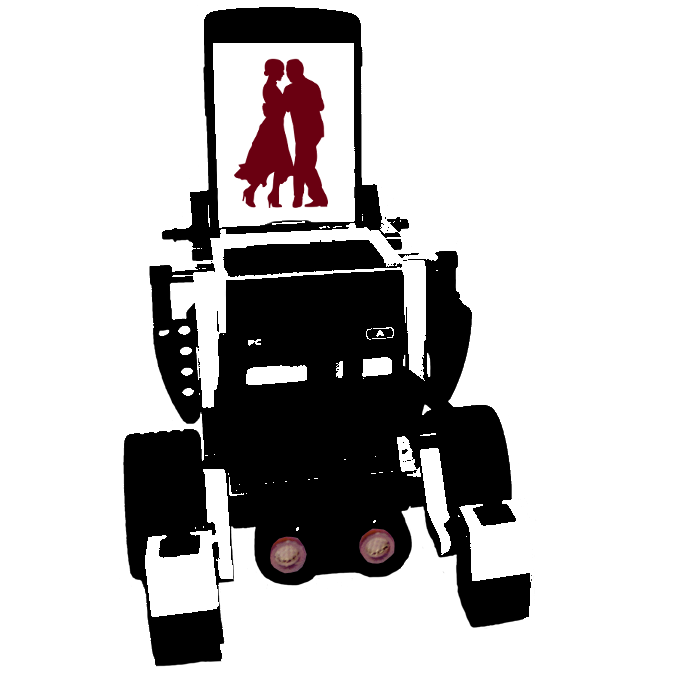
\includegraphics[width=\textwidth]{img/app_logo}	
	\end{minipage}
	
	\subsubsection{App und PC verbinden}
	Um neue Programme einfach und schnell auf das Smartphone übertragen zu können, muss zuerst das Smartphone mit dem PC verbunden werden. Dazu sind folgende Schritte nötig:
	\begin{enumerate}
	\begin{minipage}{.47\textwidth}	
	\item Starte den \textbf{Message-Server}, indem du die \textbf{ServerStarten.bat} auf dem Desktop des Computers mit einem Doppelklick ausführst. Der Server erledigt ein paar Einstellungen. Außerdem ist er später wichtig, damit die Roboter untereinander kommunizieren können.	 
	\item Um eine dauerhafte Verbindung herzustellen, müssen wir nun das Smartphone mit dem Server bekannt machen.	
	\item Der Message-Server zeigt dir links unten in der Ecke seine IP-Adresse an (siehe Screenshot auf Seit \pageref{fig:server}). Diese musst du nun der Mindroid-App mitteilen. Dazu navigierst du über das Menü oben links in den \textbf{Einstellungen-Bildschirm} (Abbildung rechts). Dort trägst du unter \textbf{MSG-Server IP} die IP des Servers ein. Ist dies erledigt, kannst du zurück zum Hauptbildschirm der App und auf \textbf{Verbinden} klicken. Die App verbindet sich nun mit dem Server.	
	\end{minipage}	
	\hfill
	\begin{minipage}{.47\textwidth}
	
	\centering
	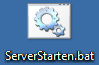
\includegraphics[width=.4\textwidth]{img/pc_serverbat.png}
	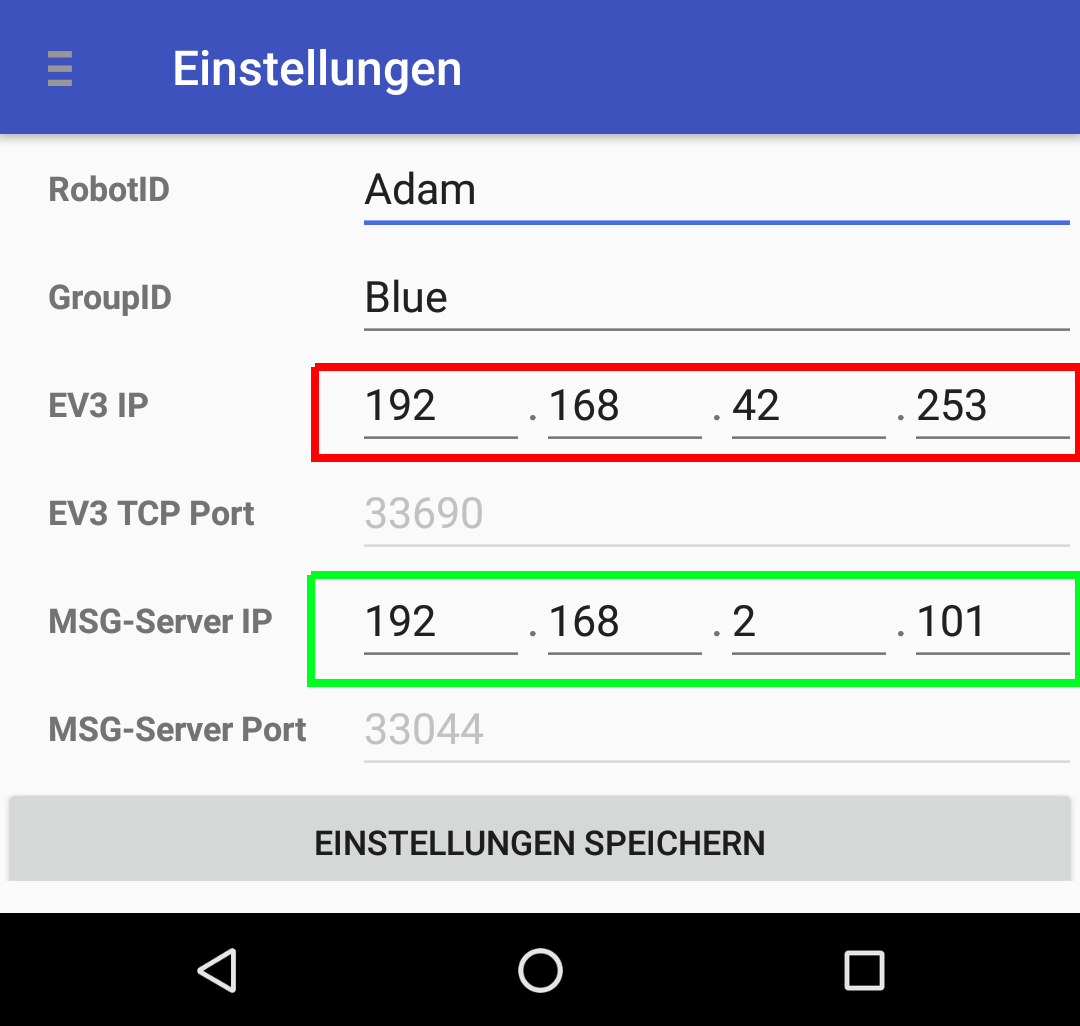
\includegraphics[width=.8\textwidth]{img/app_settings_short.png}
	\label{fig:app_settings}
	\end{minipage}
	\begin{center}
	\begin{figure}
	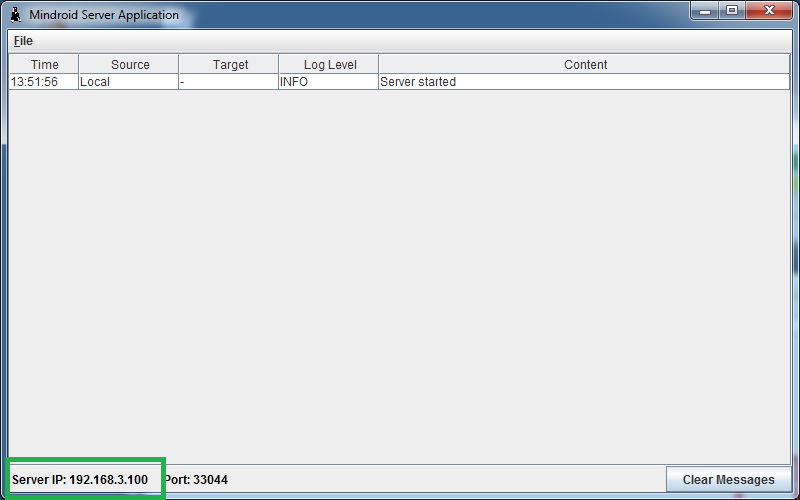
\includegraphics[width=.9\textwidth]{img/pc_server.png}
	\caption{Screenshot des Servers}
	\label{fig:server}
	\end{figure}
	
	\end{center}	

	
	
	\end{enumerate}
	
	\newpage
	
	
	\subsubsection{Programme übertragen}
	Neue Programme schreiben und übertragen wir in der	Enwicklungsumgebung \textbf{"Java-Editor"}.
	
	\begin{enumerate}
	\item Starte diesen indem du die Verknüpfung auf dem Desktop startest. In der Mitte findest du den Quelltext des aktuellen Programms, hinterlegt mit Farben, die die Orientierung erleichtern sollen.
	
	\gcenterone{img/je_main.png}
	
	Wie das Programm genau funktioniert, sehen wir uns gleich an. Zunächst einmal wollen wir es auf das Smartphone spielen, um zu sehen, was passiert.
	
	\item Dazu klickst du auf den blauen Play-Button oben links (Der Button ändert seine Farbe nach dem Durchlauf wieder zu türkis). 
	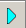
\includegraphics{img/je_playbutton.png} \\ Dein “Hallo Welt”-Programm wird jetzt an das Handy übertragen.
	
	\item In der Konsolenausgabe am unteren Bildrand sollte in etwa folgender Text erscheinen:
	\gcenterone{img/je_console.png}
	Das Programm ist nun übertragen.
	\end{enumerate}
	\newpage
	\subsubsection{Roboter und App verbinden}
	Zuletzt müssen nun noch Smartphone und Roboter miteinander verbunden werden. 
	
	
	\begin{enumerate}
	
	\begin{minipage}{.45\textwidth}
	\item Überprüfe dazu, ob wie rechts gezeigt die IP-Adresse 192.168.42.253 im Hauptmenü angezeigt wird. Ist dies nicht der Fall, folge der Anleitung in Abschnitt \ref{sec:pan} auf Seite \pageref{sec:pan}. 
	\end{minipage}
	\hfill	
	\begin{minipage}{.45\textwidth}
	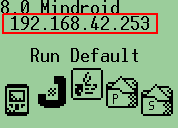
\includegraphics[width=.9\textwidth]{img/ev3_main.png}
	\end{minipage}
	
	\begin{minipage}{.45\textwidth}
	\item Wird die \textbf{IP-Adresse} im Hauptmenü des Roboters richtig angezeigt, musst du nun noch kontrollieren, ob diese IP-Adresse auch im Einstellungsmenü der App richtig gesetzt ist. Überprüfe dazu den Eintrag unter \textbf{EV3 IP}. Die farblichen Markierungen auf den Bildern sind dir dabei eine Hilfe. Falls der Eintrag nicht korrekt ist, korrigiere ihn.
	\end{minipage}	
	\hfill	
	\begin{minipage}{.45\textwidth}
	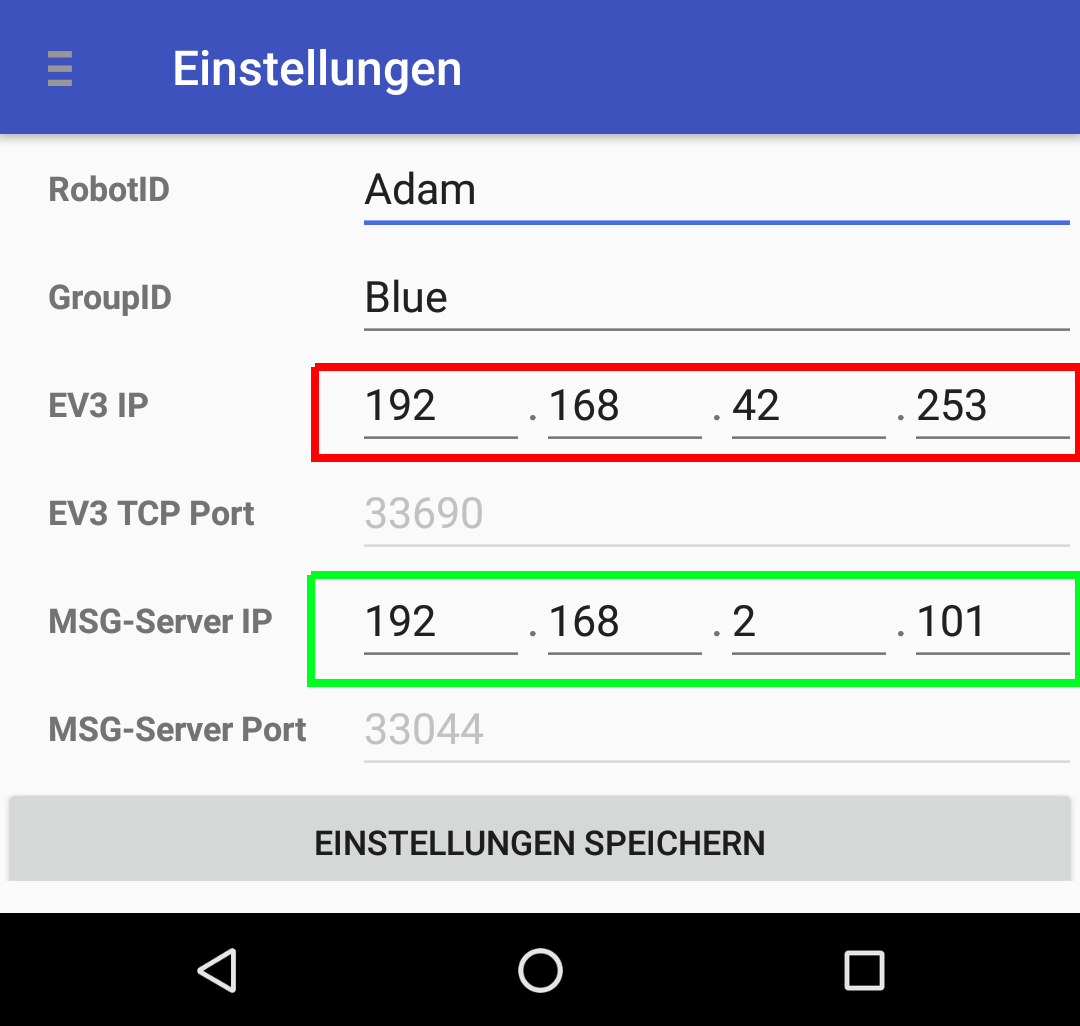
\includegraphics[width=.9\textwidth]{img/app_settings_short.png}
	\end{minipage}
	
	
	\item \label{sec:afterpan}Nun kannst du das \textbf{EV3-Programm }starten. Wähle dazu \textbf{Run Default} im Hauptmenü des Roboters aus und bestätige mit der Auswahltaste. Danach musst du warten, bis der Roboter \textbf{"Ready"} anzeigt
	
	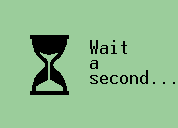
\includegraphics[width=.3\textwidth]{img/ev3_waitasecond.png}
	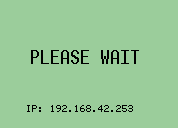
\includegraphics[width=.3\textwidth]{img/ev3_pleasewait.png}	
	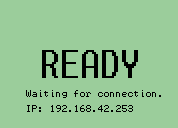
\includegraphics[width=.3\textwidth]{img/ev3_ready.png}
	\item Der Roboter ist nun bereit dazu sich mit dem Handy zu verbinden. In der App kannst du nun \glqq Verbindung zum EV3-Brick herstellen\grqq{} antippen.
	\item Um nun das Hello-World-Programm zu starten, wähle es in der Liste der App aus und drücke auf \textbf{Starten}. Es wird ausgeführt, und auf dem Bildschirm des Roboters erscheint \textbf{"Hallo Welt!"}
	
	\end{enumerate}	
	\newpage
	\subsection{Der Quelltext erklärt}
	Nachdem du den Roboter erfolgreich eingerichtet und das erste Mal getestet hast, gehen wir jetzt daran, uns den Quelltext näher anzusehen.
	\lstinputlisting{\solpath/HelloWorld.java}
	Das Verhalten des Roboters befindet sich in der \textbf{run-Methode }(Zeilen 13-16). Wenn ein Mindroid-Programm ausgeführt wird, werden die Befehle in dieser Methode nacheinander abgearbeitet.
		\begin{itemize}
		\item{\bfcode{clearDisplay()}} löscht den Display-Inhalt
		\item{\bfcode{drawString(text, textsize, xPosition, yPosition)}} schreibt einen gegebenen Text (\bfcode{text}) an die gegebenen Koordinaten (\bfcode{xPosition, yPosition}) und verwendet dabei die definierte Schriftgröße (\bfcode{textsize}).
		\item Der Konstruktor in den Zeilen 8 bis 10 gibt unserem Programm einen Namen (Zeile 8). Mit dem Aufruf von \bfcode{super("Hello World")} bestimmen wir, unter welcher Bezeichnung unser Programm später ausgewählt werden kann. Es ist sinnvoll an beiden Stellen aussagekräftige Bezeichnungen zu verwenden.
		\end{itemize}
		Daneben gibt es noch die sogenannten “\textbf{imports}”. Da die Programm-Bibliotheken der MindroidApp sehr groß sind, hat jede Klasse einen ausführlichen Namen, der dabei hilft, den Überblick zu bewahren. Der Teil vor dem Klassennamen heißt \textbf{Paket} (engl. package). Zum Beispiel ist die Klasse \textbf{ImperativeWorkshopAPI} im Paket \textbf{org.mindroid.api.}
		
		\subsection{Erste eigene Änderungen vornehmen}
		Um zu sehen, wie die Entwicklung deiner eigenen Roboter-Software im Folgenden ablaufen wird, wirst du nun am Hello-World-Programm eine kleine Änderung durchführen und anschließend das aktualisierte Programm auf den Roboter laden.
		
		Öffne dazu zuerst die \bfcode{HelloDate.java}-Datei. Ändere den Code nun, sodass er dem folgenden Code ähnelt:\\
		\textbf{Wichtig:} Ändere in keiner Aufgabe die imports oder den Package-Namen. Diese sind bereits so wie sie sein müssen.
		
		\lstinputlisting{\solpath/HelloDate.java}
		\begin{itemize}
		\item Die Imports von \bfcode{java.text.SimpleDateFormat} und \bfcode{java.util.Date} sind neu hinzugekommen.
		\item Außerdem gibt es nun eine Variable \bfcode{formatter} (Zeile 17), die in der Lage ist, das aktuelle Datum formatiert auszugeben (\bfcode{formatter.format(new Date())}, Zeile 19)).
		\end{itemize}
		Um die Änderungen nun auf das Handy zu übertragen, muss die App neu installiert werden.
		\begin{enumerate}
		\item Zuerst musst du deine Änderungen am Code 
		 speichern\footnote{Oben Links auf das Diskettensymbol klicken 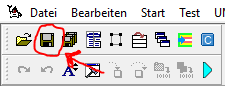
\includegraphics[]{img/je_savebutton}}. 
		\item Betätige jetzt die Schaltfläche “Starten” .
		\item Nachdem im Compiler-Fenster die Meldung “BUILD SUCCESSFUL” erschienen ist, wird auf dem Handy die Mindroid-App automatisch geschlossen und wieder geöffnet.
		\item Wähle “Verbindung zum EV3-Brick herstellen”
		\item Wähle im Dropdown “HelloWorld” aus und betätige “Start”.
		\item Auf dem Display sollte nun das aktuelle Datum ausgegeben werden.
		
		\end{enumerate}
		
	\textbf{Übrigens}\\
		
	Falls du erfahren möchtest, wie man bspw. die aktuelle Uhrzeit mithilfe von SimpleDateFormat ausgibt, klicke mit Rechts auf den Klassennamen SimpleDateFormat und wähle den Eintrag “API-Hilfe.” Im sich öffnenden Fenster findest du die Dokumentation der Formatierungsparameter, die im Konstruktor verwendet werden.
	Die vollständige Doku aller Klassen für die Mindroid-App erhältst du, indem du auf dem Desktop den Link “Mindroid Doku” anklickst.
	Die vollständige Doku aller Klassen der Java-Standardbibliothek erhältst du, indem du auf dem Desktop den Link “JDK Doku” anklickst oder die folgende URL aufrufst: https://docs.oracle.com/javase/7/docs/api/index.html 
	
	
	\section{Den Roboter kennenlernen}
	In dieser Aufgabe wollen wir gemeinsam die Fähigkeiten des Roboters kennenlernen. Das Display ist nützlich, um bestimmte Informationen schnell auszugeben, aber wirklich nützlich wird der Roboter erst durch seine beiden \textbf{Antriebsmotoren}, den \textbf{Gyrosensor}, die beiden \textbf{Lichtsensoren} und den \textbf{Ultraschallsensor}.
	
	\subsection{Fahren - die Antriebsmotoren}
	Wir schauen uns als Erstes an, wie man den Roboter fahren lassen kann. Der Roboter unterstützt folgende \textbf{Bewegungsrichtungen}:
	\begin{itemize}
	\item Vorwärts fahren,
	\item Rückwärts fahren,
	\item Drehen nach Rechts und
	\item Drehen nach Links
	\end{itemize}
	
	Um die Fahr-Fähigkeiten des Roboters kennenzulernen, wirst du den folgenden Code nachprogrammieren, der ein etwas \textbf{spezielles Quadrat} fährt.
	
	\lstinputlisting{\solpath/DriveSquare.java}
	
	\begin{itemize}
	\setlength{\itemsep}{0pt}
	\item Alle benötigten Methoden werden von der Klasse \bfcode{ImperativeWorkshopAPI} bereitgestellt. Wir brauchen daher keine zusätzlichen Imports.
	\item In Zeile 14 bestimmt die \textbf{for-Schleife}, dass der Roboter das Quadrat dreimal abfahren soll.
	\item Der \bfcode{forward()}-Befehl (Zeile 16) setzt den Roboter in Bewegung. Dabei fährt der Roboter solange, bis er einen anderslautenden Befehl erhält (wie bspw. \bfcode{stop()} in Zeile 29).
	\item Anschließend wird für 2 Sekunden \textbf{gewartet} (Zeile 16). In dieser Zeit fährt der Roboter vorwärts.
	\item Daraufhin vollführt der Roboter eine Drehung nach Rechts um 90° (\bfcode{turnRight(angle)}, Zeile 18).
	\item Nach der nächsten Geraden (Zeile 19) dreht der Roboter nach links (\bfcode{turnLeft(angle)}, Zeile 21), um anschließend die verbleibenden beiden Geraden rückwärts zu fahren (\bfcode{backward()}-Befehl, Zeile 22 und 25).
	
	\end{itemize}
	
	\subsection{Der Ultraschallsensor - Abstand Messen}
	Um dich mit dem Ultraschall-Distanzssensor vertraut zu machen, implementiere den folgenden Code nach. Er stellt einen einfachen Parksensor dar, der wie folgt funktioniert:
	\begin{enumerate}
	\item Liegt die Distanz zu einem Objekt vor dem Roboter \textbf{unter 15cm}, dann blinkt die Status-LED schnell rot und es wird “\textbf{Oh oh :-O}” ausgegeben.
	\item Liegt die Distanz \textbf{zwischen 15cm und 30cm}, dann blinkt die Status-LED gelb und es wird “\textbf{Hm :-/}” ausgegeben.
	\item Liegt die Distanz \textbf{über 30cm}, dann leuchtet die Status-LED grün und es wird “\textbf{OK :-)}” ausgegeben.
	\end{enumerate}
	
	\lstinputlisting{\solpath/ParkingSensor.java}
	
	\begin{itemize}
	\item Um die LED ansteuern zu können, müssen wir die Pakete \\ \bfcode{org.mindroid.api.ev3.EV3StatusLightColor}\\ und\\ \bfcode{org.mindroid.api.ev3.EV3StatusLightInterval} importieren.
	\item Wie in Zeile 19 zu sehen ist, läuft das Programm in einer Endlosschleife, bis der “Stop”-Knopf in der App betätigt wird.
	\item Wir müssen uns jeweils den vorherigen Zustand in der Variablen \bfcode{previousState} (Zeile 17) merken, da wir ansonsten alle 100ms den Zustand der LED zurücksetzen würden, was das Blinken verhindert. Mithilfe von \bfcode{previousState} ändern wir den LED-Modus nur dann, wenn wir müssen.
	
	\end{itemize}
	
	\subsection{Die Farbsensoren - Farbe messen}
	In dieser Aufgabe lernst du die Farbsensoren des Roboters kennen. Der folgende Quelltext liest kontinuierlich den aktuell gemessenen Farbwert des linken und rechten Lichtsensors aus (\bfcode{getLeftColor()} bzw. \bfcode{getRightColor()} in Zeilen 16 und 17).
	\\
	
	\lstinputlisting{\solpath/ColourTest.java}
	
	\begin{itemize}
	\item Die Methode \bfcode{describeColor} (Zeilen 29-39) zeigt, wie du den Rückgabewert in einen lesbaren Text umwandelst.
	\item In den Zeilen 20-21 siehst du, wie man auf dem Display mehrzeiligen Text ausgeben kann. Die Buchstaben haben jeweils eine Höhe von 16 Pixeln, sodass die zweite Zeile an der y-Position 17 und die dritte Zeile an der y-Position 33 beginnt.
	\item Um die Qualität der Farbmessung näher zu betrachten, haben wir für dich Farbtafeln mit allen sieben unterstützten Farben des EV3-Lichtsensors vorbereitet. Bei welchen Farben funktioniert die Erkennung gut, bei welchen eher weniger?
	\item Der Farbsensor kann auch zur Erkennung von Abgründen eingesetzt werden: Welche Farbwerte werden gemessen, wenn der Roboter auf der Tischplatte steht und wenn die Farbsensoren über den Tischrand ragen?
	\end{itemize}
	
	\subsection{Kommunikation zwischen Robotern} % - Verteiltes ``Hallo Welt!''}
	In der vorherigen Aufgaben hast du kennengelernt, wie ein Programm auf einem einzelnen Roboter ausgeführt wird. Als nächstes wollen wir die Roboter \textbf{miteinander sprechen lassen}.
	
	Auch hier starten wir mit einem einfachen (diesmal verteilten) “Hallo Welt!”-Programm. Die Kommunikation läuft über das bereits vorgestellten “Server”-Programm, welches ihr vorhin schon auf dem Entwicklungsrechner gestartet habt. 
	
	Damit die Roboter voneinander unterschieden werden können, benötigt jeder einen eigenen Namen. Um diese Einstellungen ändern zu können, müsst ihr die Verbindung zum Server erst einmal trennen. Navigiert nun wieder in das Einstellungs-Menü der App und gebt den Robotern Namen. Stellt sicher, dass die Roboter auch in Gruppen eingeteilt sind. 
	
	Wiederhole diesen Schritt nun auch für den zweiten Roboter. In unserem Beispiel gehen wir davon aus, die Roboter heißen Robert und Berta.
	
	Wir möchten nun, dass Berta eine Nachricht mit dem Inhalt \textbf{``Hallo Robert!''} an den Nachrichtenserver versendet. Robert soll diese Nachricht empfangen und die Nachricht auf seinem Display ausgeben. 
	Dazu sind zwei unterschiedliche Programme für Robert und Berta notwendig.
	\lstinputlisting{\solpath/HelloWorldPingB.java}
	\begin{itemize}
	\item Bei Programmstart sendet Berta in Zeile 14 eine Nachricht an \textbf{Robert }mit den Inhalt \textbf{``Hallo Robert!''}
	\end{itemize}
	
	\lstinputlisting{\solpath/HelloWorldPingR.java}
	
	\begin{itemize}
	\item Robert überprüft mit \bfcode{hasMessage()} (Zeilte 16) ob neue Nachrichten auf dem Message-Server vorhanden sind. 
	\item Sobald eine Nachricht vorliegt, wird der Inhalt der Nachricht in die Variable \bfcode{msg} gespeichert (Zeile 16).
	\item die Nachricht wird nun mit dem String \textbf{``Hallo Robert!''} verglichen\footnote{Beachte: Strings werden in Java nicht mit == verglichen, sondern mittels der \bfcode{equals()}-Methode}. Stimmen beide überein, schreibt Robert auf sein Display einen Text (Zeile 19).
	\end{itemize}
	
	\subsection{Nächste Schritte}
	Du hast jetzt alle wesentlichen Fähigkeiten des Roboters kennengelernt. Nun ist es an der Zeit, dass du deine eigenen Projekte umsetzt. Die folgenden Aufgaben geben dir dazu Anregungen.
	Falls du bestimmte Sensorwerte zur Kalibrierung nutzen willst, ist dir die Anwendung Sensor Monitoring bestimmt eine Hilfe.
	\begin{enumerate}
	\item Wähle dazu auf der Übersichtsseite des der Mindroid-App im Dropdown \textbf{“SensorMonitoring” }aus.
	\item Betätige \textbf{“Start”}.
	\item Öffne anschließend im Menü links oben den Eintrag \textbf{“Sensor Monitoring”}.
	\item Du siehst die aktuell gemessenen Werte der Sensoren
	\begin{itemize}
	
	\item Der Wert \textbf{“Color ID” }beschreibt die aktuell gemessene Farbe unter dem linken Sensor. Ihre Werte sind in der Klasse \begin{center} \textbf{org.mindroid.impl.statemachine.properties.sensorproperties.Color} 
	\end{center}dokumentiert. Wenn du ein weißes Blatt Papier direkt unter den linken Farbsensor legst, sollte der Wert auf 6 (=Weiß) wechseln (manchmal wird auch 2 (=Blau) gemessen). Wenn du einen schwarzen Gegenstand direkt unter den Sensor legst, sollte der Wert auf 1 wechseln. Die Farbbestimmung mittels Color-ID ist leider relativ unpräzise.
	\item Der Wert \textbf{“Distance“} gibt die aktuell vom Ultraschallsensor gemessene Distanz in Metern an. Bewege deine Hand vor dem Sensor vor und zurück und beobachte die Veränderung des Wertes.
	\item Der Wert \textbf{“Angle” }gibt den aktuell gemessenen Winkel des Gyro-Sensors an. Drehe den Roboter um die Hochachse und beobachte die Veränderung des Wertes.
	\end{itemize}
	\end{enumerate}
	\subsection{Nützliche Imports}
	\begin{itemize}
	\item \emph{import org.mindroid.api.ImperativeWorkshopAPI} für die Elternklasse
	\item EV3-Statuslicht:
	\begin{itemize}
	\item Farbe: \emph{import org.mindroid.api.ev3.EV3StatusLightColor;}
	\item Werte: \bfcode{EV3StatusLightColor.GREEN, .RED, .YELLOW, .OFF}
	\item Blinkhäufigkeit: \emph{import org.mindroid.api.ev3.EV3StatusLightInterval; }
	\item Werte: \bfcode{EV3StatusLightInterval.ON, .BLINKING, .DOUBLE\_BLINKING}
	\end{itemize}
	\end{itemize}
	
	\newpage
	\section{Wand-Ping-Pong}
	Nutze deine Kenntnisse, um den Roboter wie einen Ping-Pong-Ball in gerader Linie zwischen zwei Wänden/Gegenständen/... hin und her fahren zu lassen.
	Anweisungen:
	\begin{enumerate}
	\item Der Roboter soll solange geradeaus fahren, bis er eine Wand erkennt. Er soll dabei so nah wie möglich an die Wand heranfahren, ohne mit ihr zu kollidieren.
	\item Dann soll er ein kleines Stück rückwärts fahren und sich um 180° drehen
	\item Beginne bei 1.
	\end{enumerate}
	
	Bewertungskriterien:
	\begin{itemize}
	\item (1P) Ist die 180°-Drehung exakt?
	\item (1P) Vergleich: Wie nahe kommst du an die Wand heran?
	\item (1P) Vergleich: Wie schnell schaffst du eine Runde (Fahren $\rightarrow$ Wand+Drehen $\rightarrow$ Fahren)?
	\end{itemize}
	
	\section{Koordiniertes Wand-Ping-Pong}
	Diese Aufgabe lehnt sich an die vorherige an. Allerdings sollen sich nun zwei Roboter abstimmen. Beide Roboter starten nebeneinander und blicken in die gleiche Richtung.
	Anweisungen:
	\begin{enumerate}
	\item Roboter A fährt solange, bis er eine Wand entdeckt. Er setzt zurück, dreht sich um und bleibt stehen.
	\item Roboter A sendet Roboter B eine “Start”-Nachricht.
	\item Daraufhin setzt sich Roboter B in Bewegung, bis er auf die Wand trifft. Daraufhin setzt Roboter B zurück, wendet und bleibt stehen.
	\item Roboter B sendet Roboter A eine “Weiter”-Nachricht.
	\item Beginne bei 1.
	\end{enumerate}
	
	Bewertungskriterien:
	
	\begin{itemize}
	\item (1P) Roboter kollidieren nicht.
	\item (1P) Vergleich: Wie schnell schaffen die Roboter eine “Runde” (A: Fahren $\rightarrow$ Wand + Drehen + Stop; B: Warten $\rightarrow$ Fahren $\rightarrow$ Wand + Drehen + Stop)? Hier sollen die Roboter nicht möglichst nahe, sondern nahe genug an die Wand heranfahren (Abstand der Vorderachse kleiner 20cm).
	\end{itemize}
	
	\newpage
	\section{Mähroboter}
	\easygcenter{.8\textwidth}{img/task_maehroboter.jpg}
	Nutze deine Kenntnisse, um den Roboter in einem mit schwarzem (oder weißem) Klebeband abgesperrten Bereich herumfahren zu lassen (so ähnlich wie beispielsweise viele Mähroboter arbeiten).
	\begin{enumerate}
	\item Wie beim Wand Ping-Pong soll der Roboter erstmal geradeaus fahren.
	\item Wenn er eine Grenze erkennt, soll er zurücksetzen und sich eine neue Richtung aussuchen.
	\item Beginne bei 1.
	\end{enumerate}
	
	Tipp: Überprüfe, welche Color-IDs auf dem Boden und den Begrenzungen erkannt werden, um festzustellen, wann der Roboter an die Umzäunung gelangt ist.
	
	Bewertungskriterien:
	\begin{itemize}
	\item (1P) Der umgrenzte Bereich darf nicht verlassen werden! Keines der Räder darf die Umgrenzung berühren!
	\item (1P) Vergleich: Wer schafft es am schnellsten, alle vier Seiten eines viereckigen Bereichs zu “treffen”?
	\end{itemize}
	
	\newpage
	\section{Platooning}
	\easygcenter{.8\textwidth}{img/task_platooning.jpg}
	In dieser Aufgabe geht es darum, zwei Roboter hintereinander her fahren zu lassen, ohne dass es einen Auffahrunfall gibt. Aktuell forschen zahlreiche Unis und Unternehmen unter dem Schlagwort Platooning an genau dieser Problemstellung bei echten LKWs und PKWs: Die Fahrzeuge fahren dabei so nahe, dass sie den Windschatten des Vorausfahrenden ausnutzen können.
	
	Roboter A und B werden hintereinander platziert, sodass sie in die gleiche Richtung blicken. Ziel ist es zunächst, dass Roboter B den Abstand zu Roboter A in einem bestimmen Toleranzbereich hält. Die Distanzangaben im Folgenden sind nur mögliche Werte - du bestimmst selbst, was geeignete Grenzwerte sind.
	\begin{enumerate}
	\item Roboter A fährt los. Sobald der Abstand zwischen Roboter A und Roboter B größer als 35cm wird, beginnt Roboter B aufzuschließen.
	\item Wird der Abstand kleiner als 25cm, hält Roboter B die Geschwindigkeit von Roboter A .
	\item Wird der Abstand kleiner als 15cm, lässt Roboter B sich zurückfallen (oder fährt sogar rückwärts).
	\end{enumerate}
	Bewertungskriterien
	\begin{itemize}
	\item (1P) Roboter A und B fahren mind. 1 Meter hintereinander her ohne Kollisionen (weder mit anderen Robotern noch mit der Wand).
	\item (1P) Abstand bleibt in einem von euch zuvor bestimmten Bereich (Schnur), wenn beide Roboter vorwärts fahren.
	\item (1P) Vergleich: Geringstmöglicher Abstand, bei dem keine Kollision stattfindet.
	\end{itemize}
	
	\newpage
	\section{Dancing Robots}
	\easygcenter{.8\textwidth}{img/task_chachacha.png}
	Beim Cha-Cha-Cha gibt es die Tanzfigur “Verfolgung”. Dabei verfolgt jeweils ein Tanzpartner den anderen, bis beide sich umdrehen und die Rollen wechseln. Diese Figur ist tatsächlich nicht sehr weit vom Platooning-Beispiel aus der vorherigen Aufgabe entfernt.
	Der Ablauf soll dieses Mal wie folgt aussehen:
	\begin{enumerate}
	\item  Roboter A übernimmt zunächst das Kommando und fährt voraus, während Roboter B einen möglichst gleichbleibenden Abstand hält.
	\item  Roboter A beschließt nach einer gewissen Zeit, dass nun die Drehung folgt. Er stoppt und sendet eine “Drehen”-Nachricht an Roboter B.
	\item  Roboter B stoppt, wendet und sendet Roboter A eine “Gedreht”-Nachricht.
	\item  Daraufhin dreht Roboter A ebenfalls um 180°.
	\item  Nun tauschen Roboter A und B die Rollen: Roboter B fährt voraus und gibt den Ton bis zur nächsten Drehung an.
	\end{enumerate}
	Bewertungskriterien
	\begin{itemize}
	\item (1P) Einmal Verfolgung hin (Roboter A ist der Führende) und einmal Verfolgung zurück (Roboter B ist der Führende) und dabei keine Kollision!
	\item (1P) Es sollte klar erkennbar sein (bspw. per LED-Statusleuchte), wer aktuell der “Führende” ist.
	\end{itemize}
	
	\newpage
	
	\appendix
	\section{EV3 Tasten}
	Abbildung \ref{fig:buttons} zeigt dir wie die Tasten am EV3-Brick genannt werden. Die Enter-Taste wird zum Bestätigen genutzt, mit der Escape-Taste, geht es ein Menü zurück. 
		\gcenter{img/ev3_buttons.png}{EV3-Tastenbelegung\protect\footnotemark\ }{buttons}{.5\textwidth}
		\footnotetext{ Quelle http://www.ev3dev.org/images/ev3/labeled-buttons.png}
		
	Die Bedeutung der Tasten kannst du der folgenden Aufzählung entnehmen. 
	\begin{enumerate}
	\item \textbf{Escape / Zurück}
	\item \textbf{Up / Hoch}
	\item \textbf{Left / Links}
	\item \textbf{Enter / Bestätigen}
	\item \textbf{Right / Rechts}  
	\item \textbf{Down / Unten}  
	\end{enumerate}
	\newpage
	\section{PAN Einrichtung}
	\label{sec:pan}
			Wird im Hauptmenü noch nicht die richtige IP-Adresse angezeigt, müssen zuerst die PAN\footnote{PAN = Personal Area Network}-Einstellungen korrigiert werden.
		
		\begin{enumerate}	
		\begin{minipage}{.45\textwidth}
		\item Dazu musst du zuerst in das \textbf{PAN-Menü} des Roboters navigieren. Wechsle mit den Links-/Rechts-Tasten bis du den Menüpunkt \textbf{PAN} siehst und betätige die \textbf{Auswahltaste}.
		\end{minipage}
		\hfill
		\begin{minipage}{.45\textwidth}
		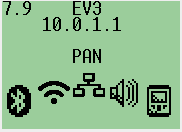
\includegraphics[width=.8\textwidth]{img/ev3_pan.png}
		\end{minipage}
		
		\item Nun navigierst du durch das Menü des Roboters wie auf den Bildern zu sehen und bestätigst jeweils mit der Auswahltaste: \textbf{USB-Client - Address - Advanced}
		
		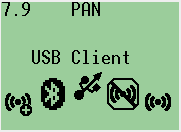
\includegraphics[width=.3\textwidth]{img/ev3_pan_usb.png}
		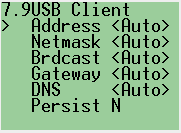
\includegraphics[width=.3\textwidth]{img/ev3_pan_usb_address.png}		
		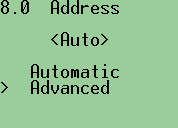
\includegraphics[width=.3\textwidth]{img/ev3_pan_usb_advanced.png}
		
		Nun musst du die IP Adresse 192.168.42.253 einstellen. Dazu navigierst du mit den rechts-/links-Tasten zu den einzelnen Ziffern und änderst deren Wert mit den oben-/unten-Tasten. Orientiere dich an den Bildern! Am Ende bestätigst du wieder mit der Enter-Taste. 
		
		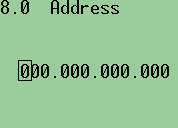
\includegraphics[width=.3\textwidth]{img/ev3_pan_usb_setip1.png}
		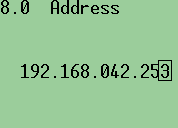
\includegraphics[width=.3\textwidth]{img/ev3_pan_usb_setip2.png}
		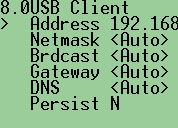
\includegraphics[width=.3\textwidth]{img/ev3_pan_usb_isset.png}
		
		\begin{minipage}{.6\textwidth}
		\item Mit der \textbf{Zurück}-Taste kommst du wieder in das Hauptmenü und die Einstellungen werden übernommen.
		\end{minipage}
		\hfill
		\begin{minipage}{.3\textwidth}
		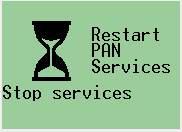
\includegraphics[width=\textwidth]{img/ev3_pan_usb_restart.png}
		\end{minipage}
		\\Nun kannst du wieder zu Punkt 3 auf Seite \pageref{sec:afterpan} wechseln.
		\end{enumerate}
		
	
	\newpage
	\section{Troubleshooting}
	\subsection{Installation über WLAN funktioniert nicht}
	Im Message-Server über \bfcode{File->Connected Devices }schauen ob alle Smartphones in der Liste auftauchen und der ADB-state auf \bfcode{connected} steht. 
	Ist dies nicht der Fall, tippe in der App auf \bfcode{TRENNEN} und stelle die Verbindung danach erneut her.
	Falls das nicht klappt, kontaktiere einen Betreuer. 
	Falls das Installieren per WLAN gar nicht mehr funktioniert, kann jederzeit eine USB-Verbindung zwischen Smartphone und PC hergestellt werden und darüber die App installiert werden.
	
	
	
	\section{Sensorbelegung}

	Tabelle	\ref{tab:sensors} zeigt die standardmäßige Sensorbelegung, wie sie in der App unter ``Mein Roboter'' definiert sein muss.
	
	\begin{table}[htbp]
		\begin{center}
		\begin{tabular}{|l|l|l|}
		\hline
		Anschluss & Sensortyp & Modus \\ \hline
		\multicolumn{1}{|r|}{1} & Farbe & ColorID \\ \hline
		\multicolumn{1}{|r|}{2} & Ultraschall & Distance \\ \hline
		\multicolumn{1}{|r|}{3} & Gyroskop & Angle \\ \hline
		\multicolumn{1}{|r|}{4} & Farbe & ColorID \\ \hline
		\end{tabular}
		\end{center}
		\caption{Sensorbelegung}
		\label{tab:sensors}
	\end{table}	
	
	Tabelle \ref{tab:motors} zeigt den standardmäßigen Motoranschluss, wie er in der App unter ``Mein Roboter'' definiert sein muss.
	\begin{table}[htbp]
		\begin{center}
		\begin{tabular}{|l|l|}
		\hline
		Anschluss & Motor \\ \hline
		A & Large Regulated Motor \\ \hline
		B & - \\ \hline
		C & - \\ \hline
		D & Large Regulated Motor \\ \hline
		\end{tabular}
		\end{center}
		\caption{Motorbelegung}
		\label{tab:motors}
	\end{table}
	
	
	
	\end{document}